% What a Bundled GNC Upgrade Hides: A Paired Ablation of a Divert-Limited
% Hit-to-Kill Interceptor.
% Build: latexmk -pdf main.tex   (figures: python make_figures.py)
% Every number in this file is traced to its source in numbers.md.
\documentclass[conference,letterpaper]{IEEEtran}

\usepackage[T1]{fontenc}
\usepackage{amsmath,amssymb}
\usepackage{graphicx}
\usepackage{booktabs}
\usepackage{xcolor}
\usepackage{tikz}
\usetikzlibrary{arrows.meta,positioning,calc}
\usepackage[hidelinks]{hyperref}
\usepackage{cite}
\usepackage{microtype}

\definecolor{ink}{HTML}{0B0B0B}
\definecolor{ink2}{HTML}{52514E}
\definecolor{ink3}{HTML}{8A8984}
\definecolor{surface}{HTML}{FCFCFB}
\definecolor{switch}{HTML}{2A78D6}
\definecolor{fixedfill}{HTML}{ECEBE7}

\newcommand{\vect}[1]{\mathbf{#1}}
\newcommand{\dv}{\Delta v}

\begin{document}

\title{What a Bundled GNC Upgrade Hides:\\A Paired Ablation of a Divert-Limited Hit-to-Kill Interceptor}

\author{\IEEEauthorblockN{Yehia Gewily}
\IEEEauthorblockA{Independent Researcher\\
Email: \href{mailto:yehiasaidgewily@gmail.com}{yehiasaidgewily@gmail.com} \quad ORCID: \href{https://orcid.org/0009-0008-3065-495X}{0009-0008-3065-495X}}}

\maketitle

\begin{abstract}
A hit-to-kill interceptor must strike its target directly, using a fixed tank of steering fuel: the divert budget.
Trade studies often compare an old guidance, navigation and control (GNC) stack against an upgraded one in which the radar, tracking filter, launch gate and guidance law all changed at once.
We show what such a bundled comparison hides, using an open simulation of a terminal interceptor.
Every parameter in it is illustrative and unclassified.
Nine configurations step from a baseline preset to an upgraded preset across the same 1000 random threats, in two atmosphere models.
As written in our baseline, proportional navigation (PN) adds a $+g$ gravity term throughout flight, which is not needed once the booster burns out and both bodies fall freely.
Dropping that coast bias saves a median 243~m/s of divert in an exponential atmosphere, and in constant-density air it raises the share of threatening threats killed from 56.8\% to 100\%.
A bundled comparison would also credit a drag-estimating filter preset, a drag-aware launch gate and a polar radar for that jump.
Tested one step at a time along our path, those three add at most 1.2 percentage points of protection.
The constant-density model also changes which upgrades look worthwhile.
Once the coast gravity bias is removed, divert use and protection remain sensitive to radar noise above the nominal specification.
The lesson: step one block at a time, on matched seeds.
\end{abstract}

\begin{IEEEkeywords}
proportional navigation, Kalman filtering, missile guidance, ablation study, paired comparison, simulation
\end{IEEEkeywords}

% =====================================================================
\section{Introduction}

A hit-to-kill interceptor carries no warhead; it destroys a threat by colliding with it head-on.
Its final stage, the kill vehicle, steers with small lateral thrusters.
Those thrusters have a fixed total velocity change to spend, which we call the \emph{divert budget} and measure in m/s.
If the kill vehicle burns through its budget before closest approach, it coasts blind for the last seconds and usually misses.

The guidance, navigation and control (GNC) loop decides how fast that budget is spent.
Think of it as a signal-processing and feedback control chain: a radar sensor feeds a tracking filter, which feeds a launch gate and a guidance controller.
Trade studies often compare a baseline GNC stack against an upgraded stack where all four blocks changed at once.
When the new stack wins, every block gets credit.
Which change actually drove the gain?
A two-stack comparison cannot tell.
We call this a \emph{bundled comparison}.

Machine learning addresses this with the ablation study~\cite{lipton2019}: you swap one block at a time along a path between configurations and measure each marginal step.
We combine this stepwise audit with \emph{common random numbers}~\cite{glasserman1992}, an established simulation variance-reduction technique.
Nine configurations, C1 to C9, walk from a baseline preset to an upgraded preset.
Every configuration flies against the exact same 1000 random threats—like testing nine receiver designs on the exact same recorded noisy waveform—so scenario-to-scenario luck cancels out of each paired contrast.

The largest effect we find is not new physics.
In our baseline preset (where boost gravity compensation carried over across stages), proportional navigation (PN) adds $+g$ to its command for the whole flight.
Once the booster burns out, the kill vehicle and threat both fall freely, so gravity cancels out of their relative motion.
Commanding $+g$ during coast acts like a DC bias in a feedback loop: it pushes the kill vehicle off its collision course, and the loop wastes divert fuel fighting its own offset.
Guidance designers know this pitfall well, and we do not present it as a discovery.
In our codebase it was fixed inside the bundled upgrade; we measure its cost in m/s and show how a bundled comparison mistakes that fix for a new filter or radar.

Our contributions are the following:
\begin{itemize}
\item \textbf{A paired stepwise audit for GNC trade studies.} We combine common random numbers with one-step-at-a-time contrasts, use a protection rate with a shared denominator, and test marginal differences with exact McNemar tests and paired bootstrap intervals.
\item \textbf{The bundled-comparison lesson.} Comparing two complete stacks credits blocks that add little or nothing under the tested configurations. This holds in both atmospheres.
\item \textbf{An atmosphere-model caution.} A drag coefficient that does not change with altitude changes which blocks appear to matter, not just the numbers.
\item \textbf{Sensitivity to radar noise.} Once the gravity bias is gone, doubling or quadrupling sensor noise above the nominal specification exhausts the divert budget and costs kills.
\end{itemize}

Section~\ref{sec:background} explains the main ideas in plain words.
Section~\ref{sec:model} describes the model, and Section~\ref{sec:design} the experiments.
Section~\ref{sec:results} gives the results.
Sections~\ref{sec:discussion} and~\ref{sec:limitations} discuss them and state the limitations.

% =====================================================================
\section{Background in Plain Words}
\label{sec:background}

\subsection{Proportional navigation and its variants}

Picture two ships on a collision course.
Seen from one ship, the other stays at a constant compass bearing; the line of sight between them does not rotate.
Proportional navigation turns this geometry into a feedback controller: it commands a sideways acceleration proportional to how fast the line of sight rotates, driving that rotation rate toward zero~\cite{murtaugh1966,shneydor1998,zarchan2012}.
The loop gain is the \emph{navigation constant}~$N$.
\emph{Augmented PN} (APN) adds a feed-forward term for a known target acceleration.
\emph{Zero-effort-miss} (ZEM) guidance expresses optimal homing laws~\cite{cottrell1971,nesline1981} by predicting the miss distance if the kill vehicle stopped steering now, and steering to cancel it~\cite{palumbo2010modern,zarchan2012}.

\subsection{Kalman filter and extended Kalman filter}

A radar measures the threat with noise.
Differentiating noisy positions directly would amplify high-frequency jitter.
A Kalman filter acts like an optimal, time-varying low-pass filter that turns noisy radar returns into a best estimate of position and velocity~\cite{kalman1960,barshalom2001}.
It also keeps a covariance matrix~$P$ that tracks how uncertain that estimate is.
At each step it predicts the next state with a motion model, then corrects the prediction with the new measurement.
The \emph{process noise}~$q$ is the random acceleration the filter expects the target to have.
In signal-processing terms, $q$ sets the filter's bandwidth: a large~$q$ follows the measurements closely, while a small~$q$ smooths them more heavily.
An \emph{extended} Kalman filter (EKF) handles a nonlinear reentry model by linearizing it around the current estimate with a Jacobian at every step~\cite{mehra1971,farina2002}.
Augmenting the state with an unknown drag coefficient is a classic EKF approach when the drag parameter is not known a priori~\cite{zarchan2009kalman,li2010survey}.

\subsection{Divert budget, predicted impact point and launch gate}

The \emph{divert} $\dv$ is the total velocity change the kill vehicle's thrusters give during its coast.
The \emph{predicted impact point} (PIP) is where the threat would hit the ground if left alone.
The \emph{launch gate} fires an interceptor only if the PIP falls inside the defended area.

\subsection{Paired seeds and the tests we use}

A \emph{seed} fixes a random scenario, so the same seed gives the exact same threat in every configuration.
For kill or no kill, only the seeds on which two configurations disagree carry information.
Let $b$ count the seeds that only the first configuration kills, and $c$ those that only the second kills (\emph{discordant} seeds).
If both designs were equally good, each disagreement would be a fair coin flip ($1/2$).
McNemar's test~\cite{mcnemar1947}, in its exact binomial form, asks how surprising the observed split $b$/$c$ is under that assumption.
This exact version is slightly conservative~\cite{fagerland2013}, so it errs on the safe side.
For divert, we take the paired difference on each seed and report its median, with a 95\% interval from a 4000-resample bootstrap~\cite{efron1979}.
Rates carry 95\% Wilson score intervals~\cite{wilson1927}.

\subsection{Is the filter honest about its own error?}

Because a simulation knows the truth, we can check the filter's reported uncertainty~$P$.
The \emph{normalized estimation error squared} (NEES) divides the squared state error by~$P$.
If the filter is honest (\emph{consistent}), its average NEES equals the number of states~\cite{barshalom2001}.
A lower value means the filter is \emph{conservative} (it claims more uncertainty than it has); a higher value means it is \emph{overconfident}.
The \emph{normalized innovation squared} (NIS) does the same check on the measurement residuals (innovations).

\subsection{Related work}

Guidance texts cover PN, APN, ZEM and optimal homing laws in depth~\cite{shneydor1998,palumbo2010modern,zarchan2012}, and earlier work examines guidance trade-offs for high-altitude and ballistic missile defence~\cite{nesline1983,zarchan1999}.
Nonlinear filtering for ballistic reentry tracking has a long history~\cite{mehra1971,farina2002,zarchan2009kalman,li2010survey}, as does the filter's role inside a homing loop~\cite{palumbo2010filter}.
Our contribution is not a new guidance law or filter.
It is an experimental method for auditing a GNC chain, and a case study of what that audit reveals.

% =====================================================================
\section{Simulation Model}
\label{sec:model}

\textbf{Every parameter in this paper is illustrative and unclassified.}
The values were chosen to make the dynamics easy to see.
They do not describe any real system.
Table~\ref{tab:params} lists the main values, and Fig.~\ref{fig:loop} shows the loop.
Appendix~\ref{app:equations} gives the remaining filter, radar and ZEM equations.

\begin{figure}[t]
\centering
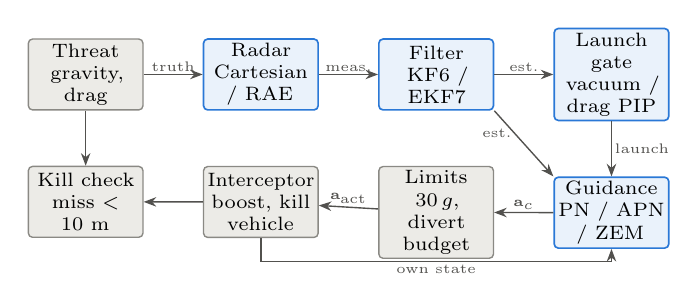
\begin{tikzpicture}[
  font=\scriptsize, >={Stealth[length=1.6mm]},
  blk/.style={draw=ink3, rounded corners=1.5pt, fill=fixedfill, align=center,
              text width=13.5mm, minimum height=9mm, inner sep=1.5pt},
  sw/.style={blk, draw=switch, fill=switch!10, line width=0.6pt},
  lab/.style={font=\tiny, text=ink2, inner sep=1pt},
  every path/.style={draw=ink2, line width=0.5pt}]
  \node[blk] (threat) {Threat\\gravity, drag};
  \node[sw, right=7.5mm of threat] (radar) {Radar\\Cartesian / RAE};
  \node[sw, right=7.5mm of radar] (filter) {Filter\\KF6 / EKF7};
  \node[sw, right=7.5mm of filter] (gate) {Launch gate\\vacuum / drag PIP};
  \node[blk, below=7mm of threat] (kill) {Kill check\\miss $<$ 10 m};
  \node[blk, below=7mm of radar] (int) {Interceptor\\boost, kill vehicle};
  \node[blk, below=7mm of filter] (lim) {Limits\\30\,$g$, divert budget};
  \node[sw, below=7mm of gate] (guid) {Guidance\\PN / APN / ZEM};
  \draw[->] (threat) -- node[lab, above] {truth} (radar);
  \draw[->] (radar) -- node[lab, above] {meas.} (filter);
  \draw[->] (filter) -- node[lab, above] {est.} (gate);
  \draw[->] (filter.south east) -- node[lab, left, pos=0.35] {est.} (guid.north west);
  \draw[->] (gate) -- node[lab, right] {launch} (guid);
  \draw[->] (guid) -- node[lab, above] {$\vect a_c$} (lim);
  \draw[->] (lim) -- node[lab, above] {$\vect a_{\mathrm{act}}$} (int);
  \draw[->] (int) -- (kill);
  \draw[->] (threat) -- (kill);
  \draw[->] (int.south) -- ++(0,-3mm) -| node[lab, below, pos=0.25] {own state} (guid.south);
\end{tikzpicture}
\caption{The engagement loop.
The radar measures the threat, and the filter estimates the threat's state.
The launch gate fires when the predicted impact point (PIP) lies inside the defended area.
The guidance law then steers the interceptor within its 30\,$g$ limit and its divert budget.
A kill is a closest approach under 10~m.
The four blue blocks are the parts that the nine configurations switch (Table~\ref{tab:configs}).}
\label{fig:loop}
\end{figure}

\begin{table}[t]
\centering
\caption{Main model parameters (all illustrative and unclassified)}
\label{tab:params}
\footnotesize
\setlength{\tabcolsep}{4pt}
\begin{tabular}{@{}ll@{}}
\toprule
Item & Value \\
\midrule
Integration & RK4, 20 ms step; flat Earth, $g = 9.81$ m/s$^2$ \\
Threat start & altitude 55--75 km, ground range 35--55 km \\
Threat flight & 70--100 s to impact; aim point within 35 km \\
Threat drag $k_T$ & $4\times10^{-5}$ m$^{-1}$ (sea-level value) \\
Atmosphere & constant density, or exponential, $H = 7$ km \\
Booster & 150 kN for 5 s, launched from the defended point \\
Kill vehicle & 200 kg, 30\,$g$ lateral limit, 435 m/s divert budget \\
Kill & closest approach under 10 m \\
Guidance & navigation constant $N = 4$ \\
Cartesian radar & 25 m, 8 m/s per axis (1$\sigma$) \\
RAE radar & 10 m, 1.2 mrad; vel.\ 3 m/s radial, 8 m/s cross \\
KF6 & no drag; $q = 30$ m$^2$/s$^3$ \\
EKF7 & estimates $k_T$; $q = 5$ m$^2$/s$^3$ \\
EKF7 drag prior & $(3.5\pm2.5)\times10^{-5}$ m$^{-1}$ \\
Launch gate & track $\ge$ 5 s, descending, $\lVert$PIP$\rVert \le 30$ km \\
\bottomrule
\end{tabular}
\end{table}

\subsection{Frame, threat and atmosphere}

The frame is flat-Earth east--north--up, with the defended point at the origin and uniform gravity.
Both bodies are point masses integrated with fourth-order Runge--Kutta (RK4) at 20~ms steps.
The threat falls under gravity and quadratic air drag:
\begin{equation}
\ddot{\vect r}_T = -g\,\hat{\vect z} - k_T\,\frac{\rho(z)}{\rho_0}\,\lVert\dot{\vect r}_T\rVert\,\dot{\vect r}_T .
\label{eq:threat}
\end{equation}
We compare two atmosphere models.
In the \emph{constant-density} model, $\rho/\rho_0 = 1$ at every height.
In the \emph{exponential} model, $\rho/\rho_0 = e^{-z/H}$ with scale height $H = 7$~km, so density falls by a factor of~$e$ every 7~km.
Intuition: in the constant model a threat at 70~km still feels sea-level air thickness, making high-altitude drag much too strong.
The exponential profile is closer to the real atmosphere at these heights~\cite{ussa1976}.
Each seed draws a starting altitude, ground range, direction, flight time and aim point (Table~\ref{tab:params}), with initial velocity $1.03\times$ the vacuum solution to the aim point.
We call a scenario \emph{threatening} if the threat, left alone, would land inside the 30~km defended radius.

\subsection{Interceptor, radar and filters}

A booster (80~m/s exit kick, 900/450~kg wet/dry, $I_{\mathrm{sp}} = 170$~s, drag $10^{-4}$~m$^{-1}$, 10\% lateral steer) gives 150~kN of thrust for 5~s.
At \emph{burnout}, its fuel runs out and the 200~kg kill vehicle (drag $8\times10^{-5}$~m$^{-1}$) separates and coasts.
It steers with lateral divert thrusters within a 30\,$g$ limit and a 435~m/s divert budget (off below 20~m range).
The radar is either \emph{Cartesian} (25~m, 8~m/s $1\sigma$ per axis) or \emph{RAE}.
The RAE radar injects polar noise in range (10~m), azimuth and elevation (1.2~mrad) and converts to Cartesian position, so angle noise turns into cross-range position noise that grows linearly with range.
For velocity, the RAE model combines a Doppler radial observation along the beam (3~m/s $1\sigma$) with synthetic cross-beam velocity observations across both transverse axes (8~m/s $1\sigma$), giving both filters a linear 6-component Cartesian observation ($H = I_6$ for KF6, $H = [I_6\;\,\vect 0]$ for EKF7).

The \emph{KF6} filter tracks position and velocity (six states).
It knows gravity, ignores drag, and uses process noise $q = 30$~m$^2$/s$^3$.
The \emph{EKF7} filter adds the drag coefficient $k_T$ as a seventh state, with prior $(3.5\pm2.5)\times10^{-5}$~m$^{-1}$ (mean $\pm$ 1$\sigma$) and $q = 5$~m$^2$/s$^3$, assuming the truth's atmosphere model.
We kept each filter as tuned in its repository preset.
Swapping KF6 for EKF7 therefore bundles $k_T$ estimation with $q = 30 \to 5$~m$^2$/s$^3$, and under APN it also activates drag feed-forward ($\hat{\vect a}_T \neq 0$).

\subsection{Launch gate}

The \emph{vacuum} PIP is the closed-form, drag-free ground crossing from the current estimate.
The \emph{drag} PIP integrates the estimate to the ground with RK4, using the EKF7's live drag estimate.
The interceptor launches once the track is 5~s old, the threat is descending, and the PIP lies within 30~km of the origin.

\begin{table}[t]
\centering
\caption{The nine configurations. Each contrast in Table~\ref{tab:contrasts} swaps one column.}
\label{tab:configs}
\footnotesize
\begin{tabular}{@{}lllll@{}}
\toprule
ID & Filter & PIP & Guidance & Radar \\
\midrule
C1 & KF6 & vacuum & PN & Cartesian \quad (baseline preset) \\
C2 & KF6 & vacuum & PN & RAE \\
C3 & EKF7 & vacuum & PN & Cartesian \\
C4 & EKF7 & drag & PN & Cartesian \\
C5 & KF6 & vacuum & APN$^{*}$ & Cartesian \\
C6 & EKF7 & vacuum & APN & Cartesian \\
C7 & EKF7 & drag & APN & Cartesian \\
C8 & EKF7 & drag & ZEM & Cartesian \\
C9 & EKF7 & drag & APN & RAE \quad (upgraded preset) \\
\bottomrule
\multicolumn{5}{@{}l@{}}{\scriptsize $^{*}$With KF6, $\hat{\vect a}_T = 0$: this is PN without the coast gravity term.}
\end{tabular}
\end{table}

\subsection{Guidance laws and the gravity term}
\label{sec:guidance}

Let $\vect r$ and $\vect v$ be the estimated threat position and velocity relative to the interceptor.
Intuition first: both bodies fall at the same rate during coast, so adding $+g$ to the command spends thruster fuel fighting nothing.
Formally, under uniform gravity the $-g\hat{\vect z}$ terms cancel in the relative acceleration:
\begin{equation}
\ddot{\vect r} = \ddot{\vect r}_T - \ddot{\vect r}_I = \vect a_{T,\mathrm{drag}} - \vect a_{I,\mathrm{drag}} - \vect a_{\mathrm{divert}} .
\label{eq:relative}
\end{equation}
With line-of-sight rotation rate $\boldsymbol\omega = \vect r\times\vect v/\lVert\vect r\rVert^2$, our baseline PN implementation commands
\begin{equation}
\vect a_c = N\,(\vect v\times\boldsymbol\omega) + g\,\hat{\vect z}
\label{eq:pn}
\end{equation}
for the whole flight.
APN keeps the $+g$ term only during boost ($\mathbb{I}_{\mathrm{boost}} = 1$), where it lofts the booster's path.
After burnout, APN drops $+g$ and instead feeds forward the estimated target drag acceleration across the line of sight, $\hat{\vect a}_{T,\perp}$:
\begin{equation}
\vect a_c = N\,(\vect v\times\boldsymbol\omega) + \tfrac{N}{2}\,\hat{\vect a}_{T,\perp} + \mathbb{I}_{\mathrm{boost}}\,g\,\hat{\vect z} .
\label{eq:apn}
\end{equation}
We call this \emph{drag feed-forward}: it steers against the threat's predicted drag before that drag shows up as line-of-sight rotation.
Because the KF6 does not estimate drag, it outputs $\hat{\vect a}_T = 0$.
APN on a KF6 (C5) is therefore exactly \emph{baseline PN without the coast gravity term}.
ZEM guidance uses the same estimate in a predicted miss (Appendix~\ref{app:equations}).

\begin{figure*}[t]
\centering
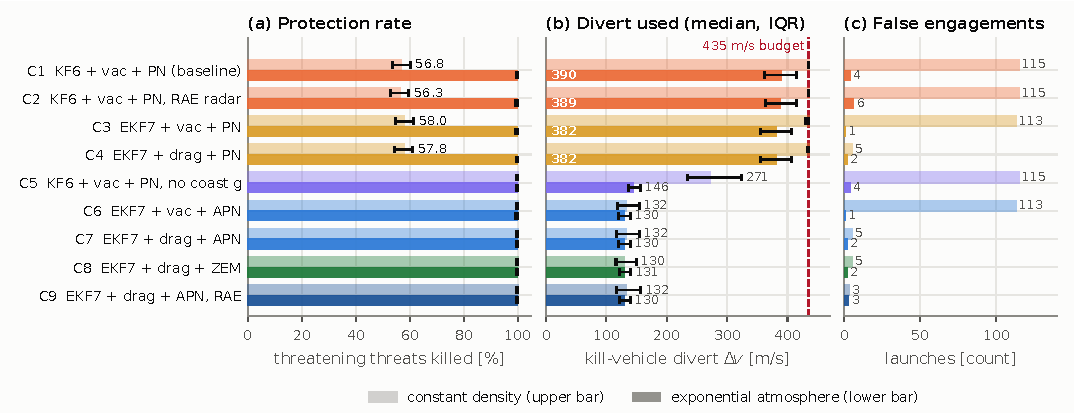
\includegraphics[width=\textwidth]{figures/ablation.pdf}
\caption{The nine-configuration ablation at the 435~m/s divert budget, 1000 paired seeds per configuration.
Each configuration has two bars: constant density (light, upper) and the exponential atmosphere (solid, lower).
(a)~Share of threatening threats killed, with 95\% Wilson intervals (845 threatening scenarios with constant density, 830 in the exponential atmosphere).
(b)~Median kill-vehicle divert over launched interceptors, with the interquartile range. The dashed line is the budget.
(c)~Launches at threats that would land outside the defended area (of 155 and 170).
With constant density, only the configurations without the coast gravity term (C5--C9) protect every threatening threat.
In the exponential atmosphere every configuration protects 99.8--100\% of threatening threats, but the gravity term still costs about 240~m/s of divert.}
\label{fig:ablation}
\end{figure*}

\begin{table*}[t]
\centering
\caption{Stepwise contrasts at the 435~m/s budget (1000 paired seeds).
Protection change in percentage points, with the discordant seeds $b$/$c$ ($b$: only the first configuration kills; $c$: only the second) and the exact McNemar $p$.
Divert change: median per-seed difference [95\% bootstrap interval], in m/s; negative means less divert.
FE: false engagements, of 155 (constant) and 170 (exponential).
The last row is the bundled comparison.}
\label{tab:contrasts}
\scriptsize
\setlength{\tabcolsep}{4pt}
\begin{tabular}{@{}l l l l l l l@{}}
\toprule
& \multicolumn{3}{c}{Constant density} & \multicolumn{3}{c}{Exponential atmosphere} \\
\cmidrule(lr){2-4}\cmidrule(l){5-7}
Change & Protection ($b$/$c$, $p$) & Divert & FE & Protection ($b$/$c$, $p$) & Divert & FE \\
\midrule
C1$\to$C2 \ Cartesian $\to$ RAE radar & $-0.5$ (14/10, 0.54) & $0.0^{\dagger}$ & 115$\to$115 & $-0.2$ (2/0, 0.50) & 0.0 & 4$\to$6 \\
C1$\to$C3 \ KF6 $\to$ EKF7 preset (with PN) & $+1.2$ (1/11, 0.006) & $0.0^{\dagger}$ & 115$\to$113 & $-0.1$ (1/0, 1.0) & $-7.7$ [$-7.9$, $-7.6$] & 4$\to$1 \\
C3$\to$C4 \ vacuum $\to$ drag PIP (PN) & $-0.2$ (2/0, 0.50) & $0.0^{\dagger}$ & 113$\to$5 & $+0.1$ (0/1, 1.0) & 0.0 & 1$\to$2 \\
\textbf{C1$\to$C5 \ drop coast gravity term} & $\mathbf{+43.2}$ \textbf{(0/365, $<10^{-100}$)} & $\mathbf{-158}$ [$-163$, $-154$]$^{\dagger}$ & 115$\to$115 & 0.0 (0/0, 1.0) & $\mathbf{-243}$ [$-245$, $-240$] & 4$\to$4 \\
C5$\to$C6 \ KF6 $\to$ EKF7 preset (with APN)$^{\ddagger}$ & 0.0 (0/0, 1.0) & $-137$ [$-141$, $-134$] & 115$\to$113 & $-0.1$ (1/0, 1.0) & $-15.2$ [$-15.4$, $-15.1$] & 4$\to$1 \\
C6$\to$C7 \ vacuum $\to$ drag PIP (APN) & 0.0 (0/0, 1.0) & 0.0 & 113$\to$5 & $+0.1$ (0/1, 1.0) & 0.0 & 1$\to$2 \\
C7$\to$C8 \ APN $\to$ ZEM & 0.0 (0/0, 1.0) & $-2.8$ [$-3.6$, $-2.1$] & 5$\to$5 & 0.0 (0/0, 1.0) & $+0.6$ [$+0.2$, $+1.2$] & 2$\to$2 \\
C7$\to$C9 \ Cartesian $\to$ RAE radar & 0.0 (0/0, 1.0) & $+0.4$ [$-0.0$, $+0.9$] & 5$\to$3 & 0.0 (0/0, 1.0) & 0.0 [$-0.4$, $+0.6$] & 2$\to$3 \\
\midrule
C1$\to$C9 \ bundled: baseline $\to$ upgraded & $+43.2$ (0/365, $<10^{-100}$) & $-297$ [$-299$, $-294$]$^{\dagger}$ & 115$\to$3 & 0.0 (0/0, 1.0) & $-259$ [$-261$, $-255$] & 4$\to$3 \\
\bottomrule
\multicolumn{7}{@{}l@{}}{\scriptsize $^{\dagger}$C1--C4 exhaust the 435~m/s budget on most seeds, capping divert. $^{\ddagger}$Under APN, KF6$\to$EKF7 combines $k_T$ estimation, $q = 30\to5$~m$^2$/s$^3$, and $\hat{\vect a}_T\neq0$.}
\end{tabular}
\end{table*}

% =====================================================================
\section{Experiment Design}
\label{sec:design}

\subsection{Nine configurations}

Table~\ref{tab:configs} lists the nine configurations.
C1 is the baseline preset, C9 is the upgraded preset, and C2--C8 form a stepping-stone path between them where each contrast swaps one column.
Because blocks can interact (for instance, EKF7's drag estimate only feeds into guidance when APN or ZEM is active), each contrast measures the marginal effect of that swap at that point along the path.
All nine share the same interceptor, threats and divert budget.

\subsection{Paired seeds and metrics}

Every configuration runs on seeds 0--999, meeting the exact same 1000 threats (845 threatening and 155 harmless with constant density; 830 and 170 in the exponential atmosphere).

Our main metric is the \emph{protection rate}: the share of threatening scenarios that end in a kill.
Its denominator is the same for every configuration.
This matters because each configuration makes its own launch choices: C1 launches at 960 threats, whereas C7 launches at only 850.
Scoring only launched interceptors would let a configuration change its own exam questions.
A \emph{false engagement} is a launch at a threat that would have landed outside the defended area.
\emph{Divert used} is the median over all launched interceptors.

\subsection{Sweeps and the filter check}

Three sweeps rerun C1, C5, C7 and C9 on the same 1000 seeds at each point (filters not retuned):
\begin{itemize}
\item the divert budget, from 100 to 550~m/s;
\item the true threat drag, from 0 to $8\times10^{-5}$~m$^{-1}$;
\item every radar noise value times 0.25, 0.5, 1, 2 or 4, at budgets of 435, 150 and 100~m/s (60{,}000 runs, exponential atmosphere only).
\end{itemize}
A companion study runs the EKF7 on 200 seeded tracking flights and computes its NEES and NIS in two settings: \emph{matched} (where the truth follows the filter's own model) and \emph{as-configured} (the ablation's settings).

\begin{figure*}[t]
\centering
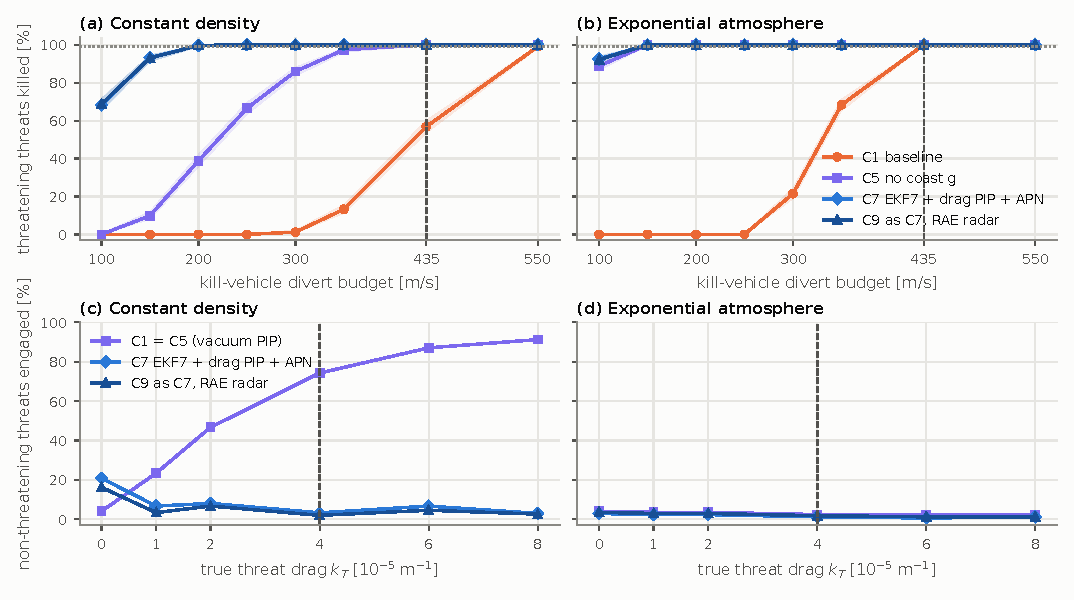
\includegraphics[width=\textwidth]{figures/sweeps.pdf}
\caption{Divert-budget and threat-drag sweeps for C1, C5, C7 and C9 (1000 paired seeds per point).
(a,~b)~Share of threatening threats killed against the divert budget, at the nominal threat drag. Bands are 95\% Wilson intervals; the dotted line marks 99\%; the dashed line is the nominal 435~m/s budget.
(c,~d)~Share of non-threatening threats engaged against the true threat drag, at the 435~m/s budget. C1 and C5 use the same vacuum PIP and launch on the same seeds.
With constant density (a,~c), the drag-aware parts in C7 and C9 lower the budget needed and prevent most false launches.
In the exponential atmosphere (b,~d), these benefits almost disappear, and the gravity term (C1 against C5) is the main difference.}
\label{fig:sweeps}
\end{figure*}

\begin{figure*}[t]
\centering
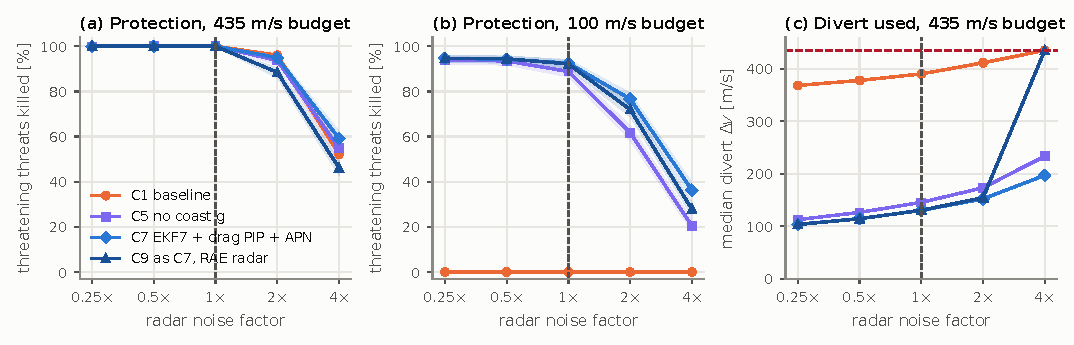
\includegraphics[width=\textwidth]{figures/noise.pdf}
\caption{Radar-noise sweep in the exponential atmosphere (1000 paired seeds per point; filters not retuned).
The noise factor multiplies every radar noise value; 1$\times$ is nominal (dashed line), where the Cartesian position noise is 25~m.
(a)~Share of threatening threats killed at the 435~m/s budget and (b)~at 100~m/s, with 95\% Wilson bands.
(c)~Median divert at the 435~m/s budget; the red line is the budget.
Divert use grows with noise in every configuration. Above 1$\times$, even the full budget no longer protects every threatening threat.}
\label{fig:noise}
\end{figure*}

\subsection{Code checks}

Step-halving tests give an observed RK4 order of 4.01 for a dragged threat and 4.00 through booster burnout.
A unit test checks that the ablation's fast engagement loop reproduces the main simulator, and every 1$\times$ run in the noise sweep matches the exponential ablation exactly.

% =====================================================================
\section{Results}
\label{sec:results}

\subsection{The coast gravity term costs divert in both atmospheres}

Fig.~\ref{fig:ablation} and Table~\ref{tab:contrasts} give the ablation.
Look first at the bold C1$\to$C5 row: it removes only the coast gravity term.

With constant density, the baseline C1 protects 56.8\% of threatening threats (480 of 845; 95\% interval 53.4--60.1\%).
Across all 960 launched flights (845 threatening plus 115 false engagements), C1 suffers 385 engaged misses (365 threatening and 20 non-threatening), all after exhausting its divert budget.
C5 protects 100\%: it rescues all 365 missed threatening seeds and loses none ($p < 10^{-100}$), cutting median divert from 435 to 271~m/s.
In the exponential atmosphere both protect every threatening threat, but median divert falls from 390 to 146~m/s—a paired saving of 243~m/s (95\% interval 240--245~m/s) that stays at 242--243~m/s across true threat drag from 0 to $8\times10^{-5}$~m$^{-1}$.

The divert-budget sweep shows how much fuel margin this buys (Fig.~\ref{fig:sweeps}a,b).
The smallest tested budget for 99\% protection falls from 550 to 435~m/s with constant density, and from 435 to 150~m/s in the exponential atmosphere.

Here is a fun control-loop question: why isn't the cost $g = 9.8$~m/s for each second of coast?
Because PN is a negative-feedback loop.
As the $+g$ bias pushes the kill vehicle off the collision course, the line of sight rotates, and PN's proportional term ($N\vect v\times\boldsymbol\omega$) pushes back to partly cancel the offset.
With constant density, on the 575 engaged seeds where both C1 and C5 kill, C1 spends a median 183~m/s more divert over a 51~s median coast—about 3.6~m/s per second of coast.\footnote{The 51~s is C5's median coast on these seeds. C1 kills earlier, after a median coast of 44~s; dividing by that gives 4.1~m/s per second. Either way, closed-loop feedback keeps the cost well under~$g$.}

\textbf{Takeaway:} removing the coast gravity term is the only change with a large effect in both atmosphere models.

\subsection{What a bundled comparison hides}

Now compare the bundled row at the bottom of Table~\ref{tab:contrasts} (C1$\to$C9) with the individual steps above it.
With constant density, the bundle raises protection from 56.8\% to 100\%, rescuing the same 365 threatening seeds as C1$\to$C5.
A bundled comparison would also credit the EKF7 preset, the drag PIP and the RAE radar.
Tested one step at a time with PN in place, those three add at most 1.2 points of protection (C1$\to$C3, $p = 0.006$), while the drag PIP (C3$\to$C4) and RAE radar (C1$\to$C2) show no significant protection change ($p \ge 0.50$).

In the exponential atmosphere, the bundle cuts median divert from 390 to 130~m/s.
Dropping the gravity term alone accounts for 243~m/s of that drop; swapping to the EKF7 preset under APN (C5$\to$C6) adds 15~m/s, and the drag PIP, ZEM and RAE radar each change divert by less than 1~m/s.

\textbf{Takeaway:} a bundled comparison credits four upgrades for a gain that mostly comes from one.

\subsection{The atmosphere model changes the conclusion}

With constant density, the drag-aware blocks look valuable once the gravity bias is gone (Fig.~\ref{fig:sweeps}a,c).
Swapping KF6 for the EKF7 preset under APN (C5$\to$C6, combining $k_T$ estimation, $q = 30\to5$~m$^2$/s$^3$, and APN drag feed-forward) saves another 137~m/s, so C7 needs a median of 132~m/s and lowers the 99\%-protection budget from 435 to 200~m/s (where C5$\to$C7 rescues 514 seeds and loses none).
Meanwhile, the drag PIP (C6$\to$C7) cuts false engagements from 113 to 5 of 155 ($p = 6\times10^{-33}$); without it, false engagements reach 91\% of non-threatening threats at $8\times10^{-5}$~m$^{-1}$ because a dragged threat falls short of the vacuum parabola.

The exponential atmosphere tells a different story (Fig.~\ref{fig:sweeps}b,d).
For C7, intercepts occur at a median altitude of 34.5~km (range 25--43~km), where air density is under 1\% of its sea-level value.
Up to intercept, the threat flies in near-vacuum: false engagements stay at 1--6 of 170 across all configurations, and sweeping true threat drag from 0 to $8\times10^{-5}$~m$^{-1}$ leaves protection (99.9--100\%) and median divert (within 1~m/s) virtually unchanged.
The C5$\to$C6 filter swap saves only 15~m/s, which we have not split between drag feed-forward and the EKF7 preset's lower velocity error (2.0~m/s median RMS velocity error vs.\ 3.1~m/s for KF6).
Still, that 15~m/s margin decides kills at a tight 100~m/s budget, where C7 protects 92.5\% and C5 88.8\% (rescuing 34 seeds vs.\ 3 lost, $p = 1.2\times10^{-7}$).

\begin{figure}[t]
\centering
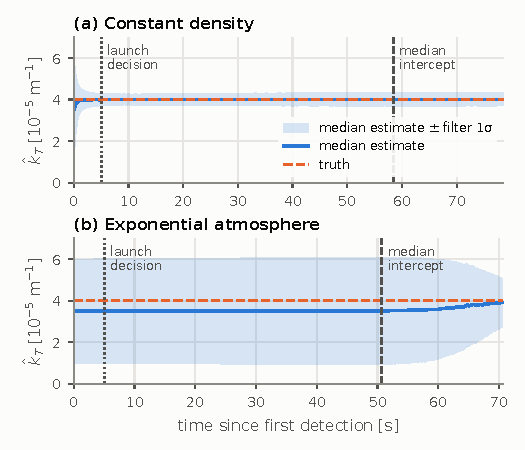
\includegraphics[width=\columnwidth]{figures/drag_estimate.pdf}
\caption{The EKF7's drag estimate over 200 seeded tracking runs, as configured (RAE radar, true $k_T = 4\times10^{-5}$~m$^{-1}$).
The line is the median estimate, the band the filter's own median 1$\sigma$, and the dashed line the truth.
Dotted: launch decision at 5~s. Dashed: median intercept time.
(a)~With constant density, the filter learns the drag before the launch decision.
(b)~In the exponential atmosphere the estimate is still at its prior at the median intercept, because thin air shows almost no drag.}
\label{fig:drag}
\end{figure}

The filter study reveals the signal-to-noise mechanism (Fig.~\ref{fig:drag}).
Intuition: a filter can only learn drag where the air is thick enough to produce a deceleration signal above radar noise.
With constant density, the EKF7 locks onto $k_T$ before the 5~s launch decision: its median estimate is $3.99\times10^{-5}$~m$^{-1}$ against a truth of 4.0 (about 1\% median absolute error).
In the exponential atmosphere, the estimate is still stuck at its prior at the median intercept time ($3.51\times10^{-5}$ vs.\ a prior of 3.5), and its 1$\sigma$ band has not shrunk (2.58 vs.\ 2.5).
The drag-aware blocks are then running on their hardcoded prior, not on live measurements.

\textbf{Takeaway:} with an altitude-independent drag coefficient the drag-aware blocks look valuable; in the exponential atmosphere they matter only at a tight budget.

\subsection{Sensitivity to radar noise}
\label{sec:noise}

Fig.~\ref{fig:noise} plots the radar-noise sweep.
Because guidance multiplies line-of-sight rate jitter by $N = 4$, divert use grows with noise in every configuration: C7 at 435~m/s uses a median 104, 130, 152 and 197~m/s at 0.25$\times$, 1$\times$, 2$\times$ and 4$\times$ noise.
Above nominal noise, even the full 435~m/s budget no longer protects every threat: at 2$\times$, 4--12\% of threatening threats leak through, and at 4$\times$, 41--54\%, with every miss exhausting its divert budget.
Below 1$\times$ little changes (at 100~m/s, C7 edges up only from 92.5\% to 94.7\%), so nominal noise sits right at the knee where noise begins to cost kills.

The gravity term stays the largest divert sink among the tested GNC changes, costing 253~m/s at 0.25$\times$ and 192~m/s at 4$\times$.
At 4$\times$ noise and 435~m/s, however, C1 and C5 protect about equally (52.2\% and 54.8\%, $p = 0.29$) because noise saturates both.
At 2$\times$, C1 kills slightly more than C5 (46 vs.\ 27 discordant seeds, $p = 0.034$); we have not established why.

Meanwhile, C7's edge over C5 grows with noise: at 100~m/s it rises from 3.7 points at 1$\times$ to 15.8 points at 4$\times$ (36.3\% vs.\ 20.5\%), and the drag PIP holds false engagements at 4--5 of 170 while the vacuum PIP rises to 13--19.
Here, signal-processing discipline prevents a false claim.
Switching from C5 to C7 also lowers the filter's process noise ($q = 5$ vs.\ 30~m$^2$/s$^3$), narrowing its bandwidth so it smooths noisy measurements more heavily.
Because the drag estimate barely leaves its prior in this atmosphere (Fig.~\ref{fig:drag}b), the lower $q$ is the more likely cause of the gain.
We have not tested this separately, and we do not credit drag estimation for it.

At high noise the RAE radar trails the Cartesian radar, losing 6.5 points at 2$\times$ and 13.0 points at 4$\times$ (C7$\to$C9 at 435~m/s; $p = 1.2\times10^{-8}$ and $4.9\times10^{-10}$).
This comes from beam geometry under our noise settings: at the 72--86~km slant range where tracking starts, 1.2~mrad of angle noise already translates to 85--105~m of cross-range position noise, against 25~m for the Cartesian radar.
Multiplying both by the same noise factor penalizes the wide cross-range axis harder; it does not show that polar radars are worse in general.

\textbf{Takeaway:} above the nominal noise, radar noise limits every configuration, even at the full budget.

\subsection{Small or no observed effects, and filter honesty}

At nominal noise, two swaps show no observed protection difference (0/0 discordant seeds) and only small or near-zero divert changes: ZEM instead of APN (C7$\to$C8) changes median divert by $-2.8$~m/s [$-3.6$, $-2.1$] with constant density and $+0.6$~m/s [$+0.2$, $+1.2$] in the exponential atmosphere (under 3~m/s), with identical false engagements; the RAE radar instead of the Cartesian one (C7$\to$C9) changes median divert by less than 1~m/s and false engagements by at most 2.
A nonsignificant test indicates no detected difference on 1000 seeds rather than strict equivalence.

The consistency study confirms that the EKF7 is honest when matched to its own model (constant density): its mean 7-state NEES is 7.08, with 94.0\% of steps inside the 95\% bounds [6.49, 7.53], and its mean NIS is 6.00 for 6 measurements.
As configured in the ablation, the EKF7 is conservative, with a mean NEES around 4.5 against an expected 7 (4.55 in constant density, 4.57 in the exponential atmosphere), because it budgets for random target acceleration and drag drift that the nominal threat does not have.
We left it un-retuned so the ablation reflects the shipped presets.

% =====================================================================
\section{Discussion}
\label{sec:discussion}

\textbf{Step one block at a time, on paired seeds.}
A stepwise ablation measures the marginal effect of each swap under the tested configurations (noting that blocks interact, and even our KF6$\to$EKF7 preset swap bundled $q = 30\to5$~m$^2$/s$^3$ with drag estimation).
Common random numbers~\cite{glasserman1992} shrink the 95\% interval on the 243~m/s gravity saving to $\pm$2~m/s, while a shared denominator keeps launch-gate differences from skewing the score.

\textbf{Check the atmosphere model before trusting a drag result.}
With constant density, our study would recommend online drag estimation, drag feed-forward and a drag-integrated PIP.
In the exponential atmosphere, those blocks matter mainly at a tight budget because high-altitude drag sits below the noise floor until after intercept.
A trade study can solve its equations right and still mislead about the world.

\textbf{Margins near the nominal noise are thin.}
Doubling the radar noise lets 4--12\% of threatening threats leak through even at the full budget.

\textbf{What we do not claim.}
The gravity-term result measures the cost of a known textbook pitfall; it is not a discovery.
We also do not claim that drag-model mismatch limits performance: C5 knows nothing about drag, yet protects at least 99.9\% of threatening threats across every tested drag value in both atmospheres.

% =====================================================================
\section{Limitations}
\label{sec:limitations}

\begin{itemize}
\item The Earth is flat, gravity is uniform, and both bodies are point masses with no seeker or attitude loop; a kill is purely geometric ($< 10$~m).
On a spherical Earth, gravity differs slightly between the two bodies, leaving a small differential gravity term during coast.
\item Drag does not depend on the Mach number, and the exponential atmosphere uses a single fixed scale height ($H = 7$~km).
\item The RAE radar converts polar position to Cartesian coordinates and supplies synthetic cross-beam velocity observations (8~m/s $1\sigma$) so both filters use a linear Cartesian measurement update ($H = I_6$ for KF6, $H = [I_6\;\,\vect 0]$ for EKF7).
\item Filters were not retuned for the sweeps, and KF6$\to$EKF7 changes both state dimension and process noise ($q = 30\to5$~m$^2$/s$^3$).
\item The radar-noise sweep was run in the exponential atmosphere only.
\item With constant density and a drag-free threat ($k_T = 0$), the drag PIP launches at more non-threatening threats than the vacuum PIP (36 vs.\ 7 of 173, $p < 10^{-8}$) due to a one-sided spread of short predictions, consistent with the EKF7 clipping $\hat k_T \ge 0$; no unclipped run has tested that explanation.
\item All results come from one scenario distribution.
\end{itemize}

% =====================================================================
\section{Conclusion}

We stepped one GNC block at a time in a divert-limited interceptor simulation, across 1000 paired seeds and two atmosphere models.
Removing our baseline PN's coast gravity bias is the only change with a large payoff in both.
A bundled comparison of the two presets credits blocks that add little under the tested configurations, while a constant-density drag model makes drag estimation look far more observable than it is in thinning air.
Once the gravity bias is removed, divert use and protection remain sensitive to radar noise above the nominal specification.
We hope this case study and the open code help others audit GNC chains cleanly.

% =====================================================================
\section*{Code and Data Availability}

The simulator, configs, result files (\nolinkurl{results/}), equations (\nolinkurl{docs/methods.md}), study scripts (\nolinkurl{scripts/ablation_study.py}, \nolinkurl{scripts/sensitivity_study.py}, \nolinkurl{scripts/ekf7_consistency.py}), manuscript source (\nolinkurl{paper/main.tex}), traceability table (\nolinkurl{paper/numbers.md}, checked by \nolinkurl{paper/check_numbers.py}) and figure script (\nolinkurl{paper/make_figures.py}) for this work are available in the companion THAAD-Simulation repository and archived on Zenodo (doi \href{https://doi.org/10.5281/zenodo.24208791}{10.5281/zenodo.24208791}; data and simulator release v1.1.0 at doi \href{https://doi.org/10.5281/zenodo.24311162}{10.5281/zenodo.24311162}).
All parameters are illustrative and unclassified.

\bibliographystyle{IEEEtran}
\bibliography{refs}

\appendices

\section{Further Equations}
\label{app:equations}

\textbf{ZEM guidance.} With time to go $t_{go} = -\vect r\cdot\vect v/\lVert\vect v\rVert^2$, the predicted miss is $\vect{Z} = \vect r + \vect v\,t_{go} + \tfrac12\hat{\vect a}_T\,t_{go}^2$.
The command is $\vect a_c = (N/t_{go}^2)\,\vect Z_\perp + \mathbb{I}_{\mathrm{boost}}\,g\,\hat{\vect z}$, where $\vect Z_\perp$ is the part of $\vect Z$ across the line of sight.

\textbf{Actuator limits.} Every law is limited to $\lVert\vect a_{\mathrm{act}}\rVert \le 30\,g$, and the divert used, $\int_{t_b}^{t}\lVert\vect a_{\mathrm{act}}\rVert\,d\tau$ after burnout time $t_b$, may not exceed the 435~m/s budget.

\textbf{EKF7.} The state is $[\vect r, \vect v, k_T]$ with $6\times7$ measurement matrix $H = [I_6\;\,\vect 0]$ and dynamics
\begin{equation*}
\dot{\vect v} = -g\hat{\vect z} - k_T\,\frac{\rho}{\rho_0}\lVert\vect v\rVert\vect v, \qquad \dot k_T = 0,
\end{equation*}
plus a random walk on $k_T$ ($q_{\mathrm{drag}} = 10^{-12}$~m$^{-2}$s$^{-1}$, clipped to $[0, 5\times10^{-4}]$~m$^{-1}$).
The state uses RK4; covariance uses $\Phi = I_7 + F\Delta t + \tfrac12(F\Delta t)^2$ from the analytical Jacobian, with
\begin{align*}
\frac{\partial\dot{\vect v}}{\partial\vect v} &= -k_T\,\frac{\rho}{\rho_0}\Bigl(\lVert\vect v\rVert I_3 + \frac{\vect v\vect v^\top}{\lVert\vect v\rVert}\Bigr),\\
\frac{\partial\dot{\vect v}}{\partial k_T} &= -\frac{\rho}{\rho_0}\,\lVert\vect v\rVert\vect v .
\end{align*}
In the exponential atmosphere it also has an altitude term, $\partial\dot{\vect v}/\partial z = (k_T/H)\,e^{-z/H}\lVert\vect v\rVert\vect v$.
Both filters use the Joseph form of the covariance update to keep $P$ symmetric and positive definite in floating-point arithmetic~\cite{barshalom2001}.

\textbf{RAE radar.} At the measured range $r$, elevation $\phi$ and beam unit vectors $\vect u_r, \vect u_\theta, \vect u_\phi$, the $6\times6$ covariance is $\operatorname{diag}(R_p, R_v)$ with position block
\begin{equation*}
R_p = \sigma_r^2\vect u_r\vect u_r^\top + \sigma_{\mathrm{az}}^2\vect u_\theta\vect u_\theta^\top + \sigma_{\mathrm{el}}^2\vect u_\phi\vect u_\phi^\top ,
\end{equation*}
and velocity block $R_v = \sigma_{\dot r}^2\vect u_r\vect u_r^\top + \sigma_{v_\perp}^2(\vect u_\theta\vect u_\theta^\top + \vect u_\phi\vect u_\phi^\top)$, where $\sigma_{\mathrm{az}} = \max(r\lvert\cos\phi\rvert\,\sigma_\theta, \sigma_r)$ and $\sigma_{\mathrm{el}} = \max(r\,\sigma_\phi, \sigma_r)$ are floored at $\sigma_r = 10$~m, $\sigma_{\dot r} = 3$~m/s is Doppler noise, and $\sigma_{v_\perp} = 8$~m/s is synthetic cross-beam velocity noise.

\textbf{Kill check.} Within each step, both bodies move along straight chords.
The closest approach on the chords decides the kill (under 10~m).
The chord departs from the true path by at most $a\Delta t^2/8$, about 1.5~cm at 30\,$g$.

\end{document}
